%Modo presentación
\documentclass[12pt]{beamer}

%Modo handout
%\documentclass[handout,compress]{beamer}
%\usepackage{pgfpages}
%\pgfpagesuselayout{4 on 1}[border shrink=1mm]

\usepackage{graphicx}
\usepackage{beamerthemeCambridgeUS}
\usepackage{ragged2e}
\usepackage{multimedia}
\usepackage{subfig}
\usepackage{tikz}
\usepackage{amsmath}
\setbeamercovered{transparent}
\usepackage{textpos} 

\title[Ambiente de Trabajo]{ANÁLISIS GEOESPACIAL}
\author[Edier Aristizábal]{Edier V. Aristizábal G.}
\institute{\emph{evaristizabalg@unal.edu.co}}
\date{(Versión:\today)}
\usepackage{textpos} 

\graphicspath{{G:/My Drive/FIGURAS/}}

\addtobeamertemplate{headline}{}{%
	\begin{textblock*}{2mm}(.9\textwidth,0cm)
	\hfill
\includegraphics[height=1cm]{logo3}  
	\end{textblock*}
			}
%############################INICIO#############################################
\begin{document}
\begin{frame}
\titlepage
\centering
	
\includegraphics[width=5cm]{unal.png}\hspace*{4.75cm}~%
   	
\includegraphics[width=2cm]{unal} 
\end{frame}
 %#############################SLIDE
\begin{frame}
\frametitle{}
\centering
	\includegraphics[width=9cm]{pythonvsR} 
\end{frame}
 %#############################SLIDE
\begin{frame}
\frametitle{}
\centering
	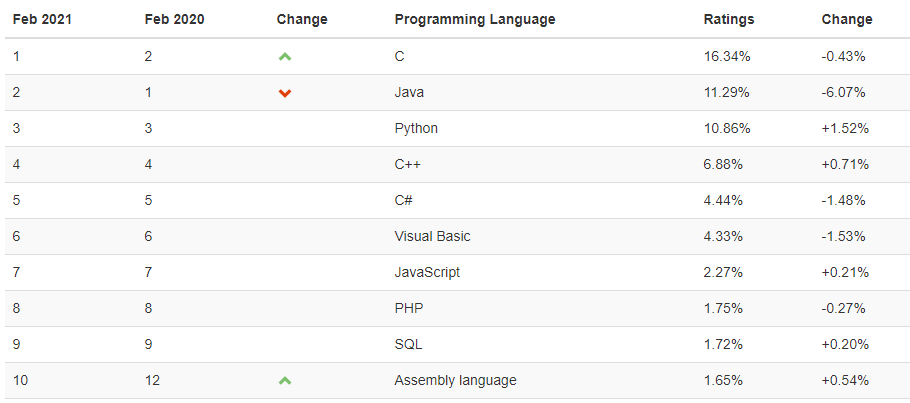
\includegraphics[width=9cm]{tiobe} 
\end{frame}
%#############################SLIDE
\begin{frame}
\scriptsize {
\alert{Python code is fast to develop}: As the code is not required to be compiled and built, Python code can be much readily changed and executed. This makes for a fast development cycle.\vfill
\alert{Python code is not as fast in execution}: Since the code is not directly compiled and executed and an additional layer of the Python virtual machine is responsible for execution, Python code runs a little slow as compared to conventional languages like C, C++, etc.\vfill
\alert{It is interpreted}: Many programming languages require that a program be converted from the source language, such as C++ or Visual Basic, into binary code that the computer can understand. This requires a compiler with various options. Python is an interpreted language, which means it does not need compilation to binary code before it can be run. You simply run the program directly from the source code, which makes Python easier to work with and much more portable than other programming languages.\vfill
\alert{It is object oriented}: Python is an object-oriented programming language. An object--oriented program involves a collection of interacting objects, as opposed to the conventional list of tasks. Many modern programming languages support object-oriented programming. ArcGIS and QGIS is designed to work with object-oriented languages, and Python qualifies in this respect.
}
\end{frame} 
%################################SLIDE
\begin{frame}
\scriptsize{\alert{An interpreter} reads a high-level program and executes it, meaning that it does what the program says. It processes the program a little at a time, alternately reading lines and performing computations.}\\
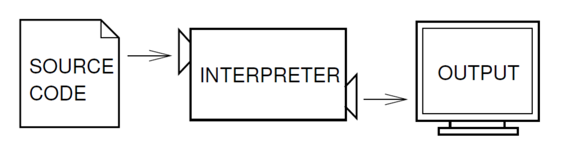
\includegraphics[width=8cm]{source}\\
\vfill
\scriptsize{\alert{A compiler} reads the program and translates it completely before the program starts running.
In this context, the high-level program is called the source code, and the translated program is called the object code or the executable. Once a program is compiled, you can execute it repeatedly without further translation.} 
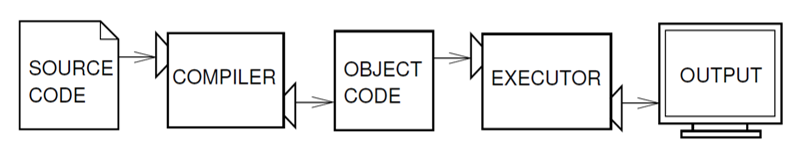
\includegraphics[width=10cm]{source1}
\end{frame} 
%############################SLIDE
\begin{frame}
\frametitle{}
\centering
	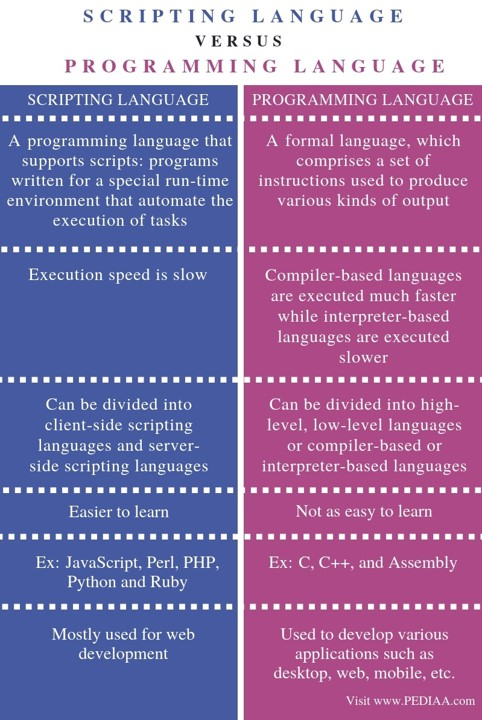
\includegraphics[width=5cm]{scriptingvsprogram} 
\end{frame}
%#############################SLIDE 
\begin{frame}
\frametitle{}
\centering
	
\includegraphics[width=12cm]{python2vspython3}
\vfill
\url{https://wiki.python.org/moin/Python2orPython3}
\end{frame}
%#############################SLIDE
\begin{frame}
\frametitle{}
\centering
	
\includegraphics[width=12cm]{anaconda}
\vfill
\url{https://www.anaconda.com/download/}
\end{frame}
%#############################SLIDE 
\begin{frame}
\frametitle{}
\centering
	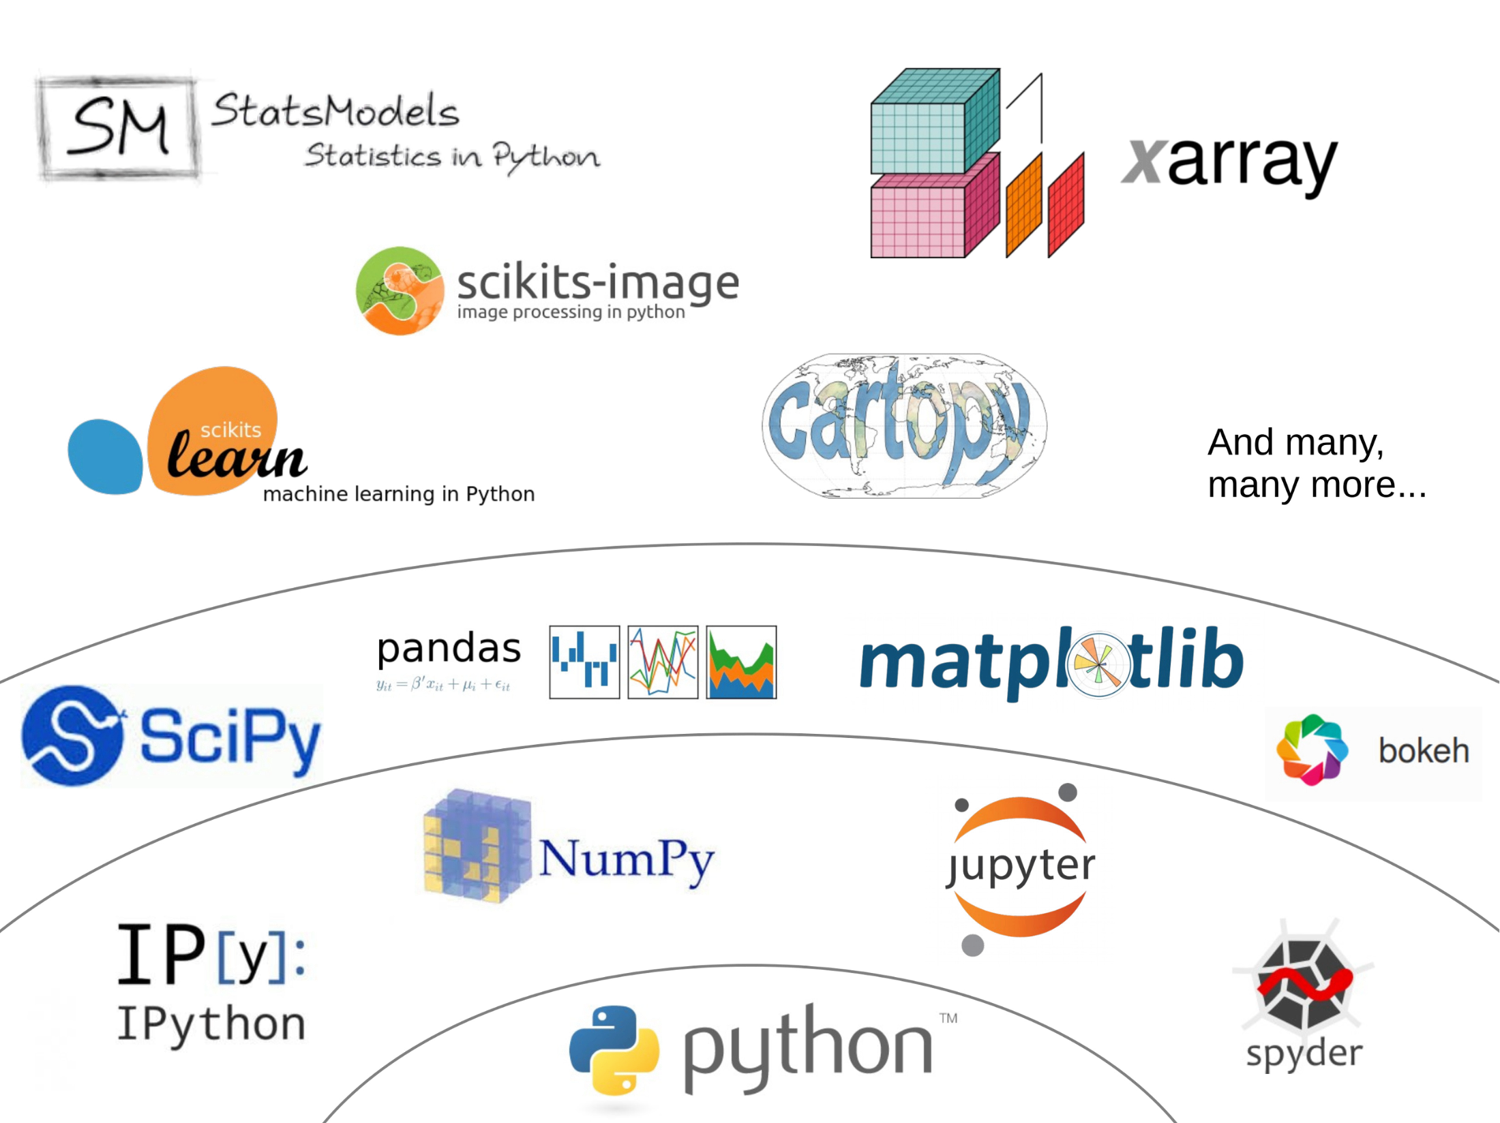
\includegraphics[width=12cm]{paquetes}
\end{frame}
%#############################SLIDE
\begin{frame}
\frametitle{}
\centering
	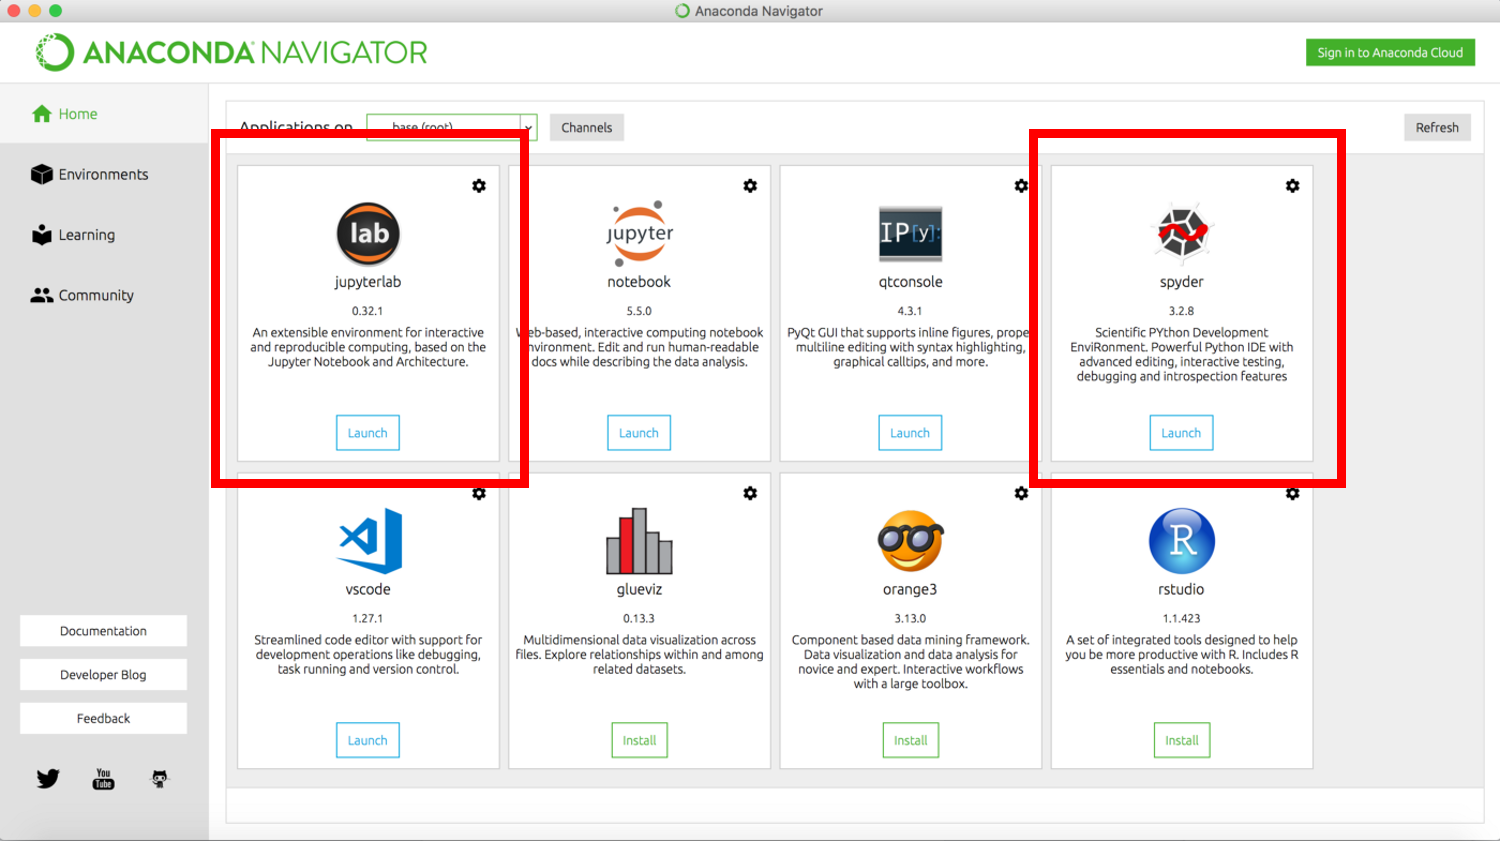
\includegraphics[width=12cm]{anacondanav}
\end{frame}
%#############################SLIDE 
\begin{frame}
\frametitle{}
\centering
	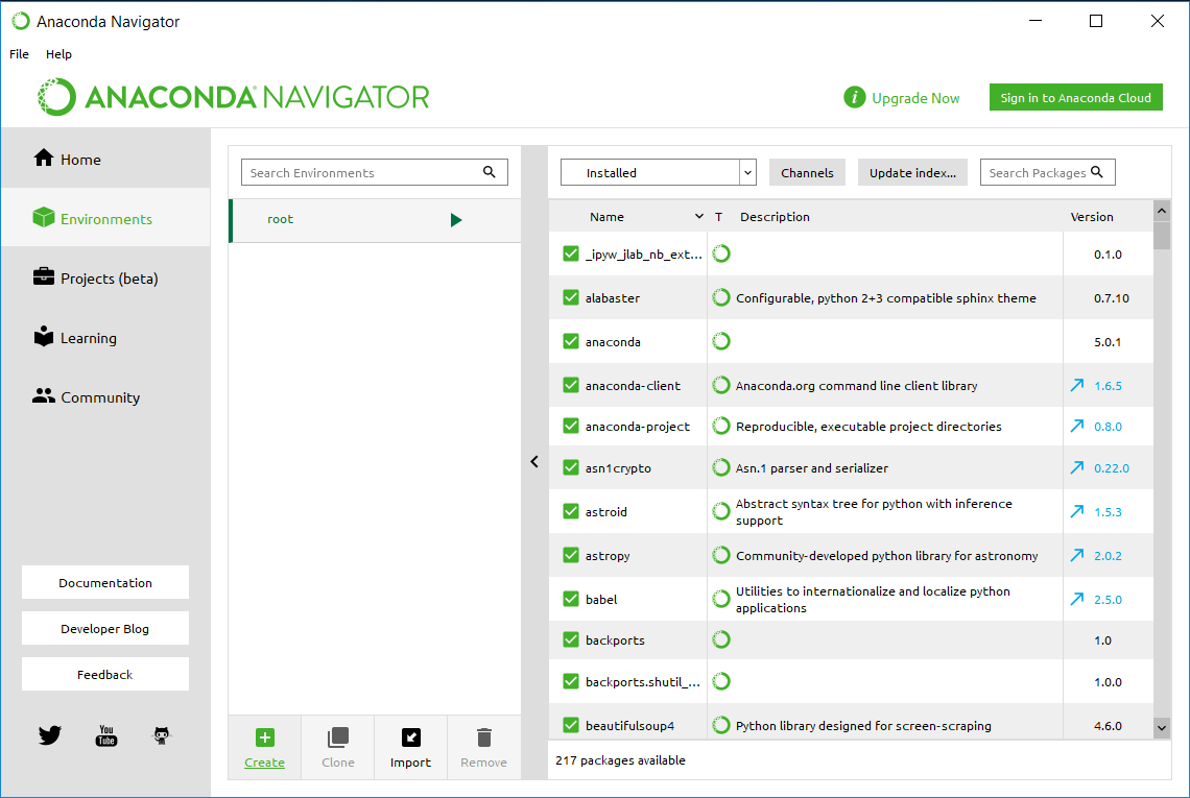
\includegraphics[width=12cm]{anaco}
\end{frame}
%#############################SLIDE 
\begin{frame}
 \begin{center}
        \begin{tikzpicture}
            \node[anchor=south west,inner sep=0] (image) at (0,0) {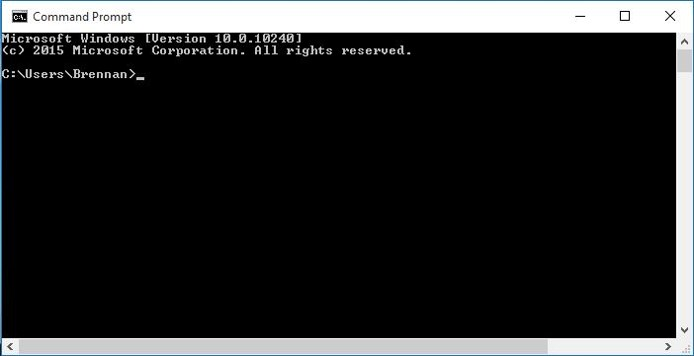
\includegraphics[width=1.4\textheight]{cmd}};
            \node[align=center,white,font={\small\bfseries}] at (image.center) {conda create xxxx\\ conda activate xxxx\\ deactivate\\ conda intall xxxx\\ conda uninstall xxx\\ conda update xxx};
        \end{tikzpicture}
    \end{center}
\end{frame}
%#############################SLIDE 
\begin{frame}
\frametitle{Python Packaging Index}
\centering
	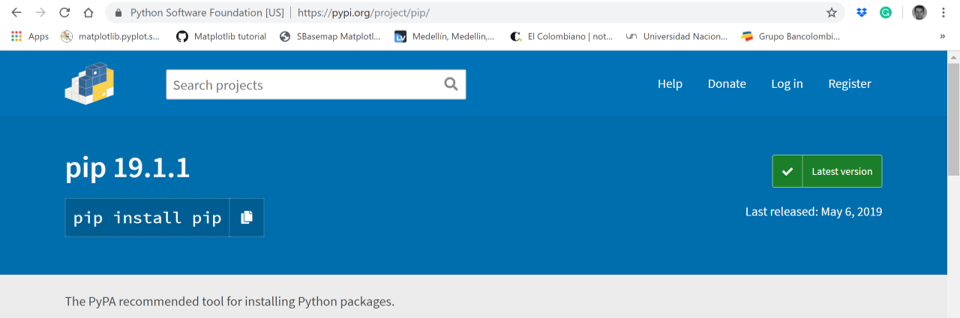
\includegraphics[width=12cm]{pip}
\vfill
\url{https://pypi.org/project/pip/}
\end{frame}
%#############################SLIDE 

\begin{frame}
\frametitle{Python}
\centering
	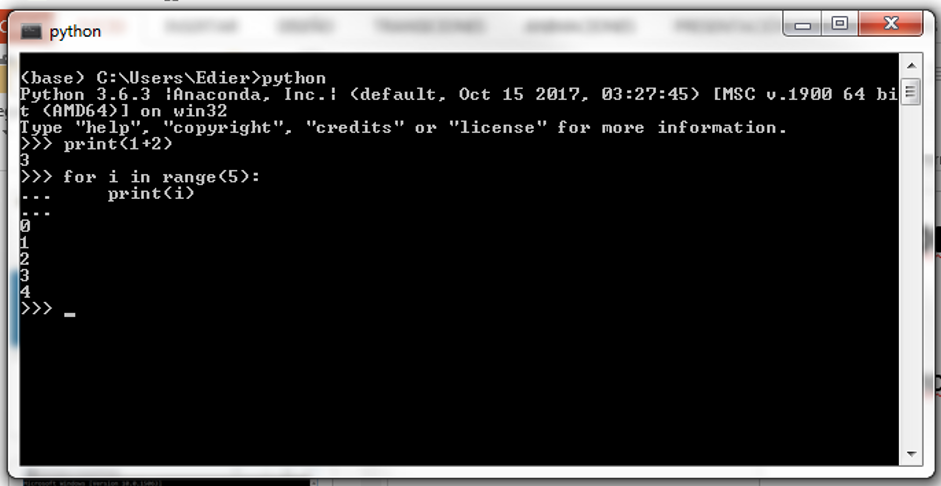
\includegraphics[width=12cm]{repl}
\end{frame}
%#############################SLIDE 
\begin{frame}
\frametitle{IPython}
\centering
	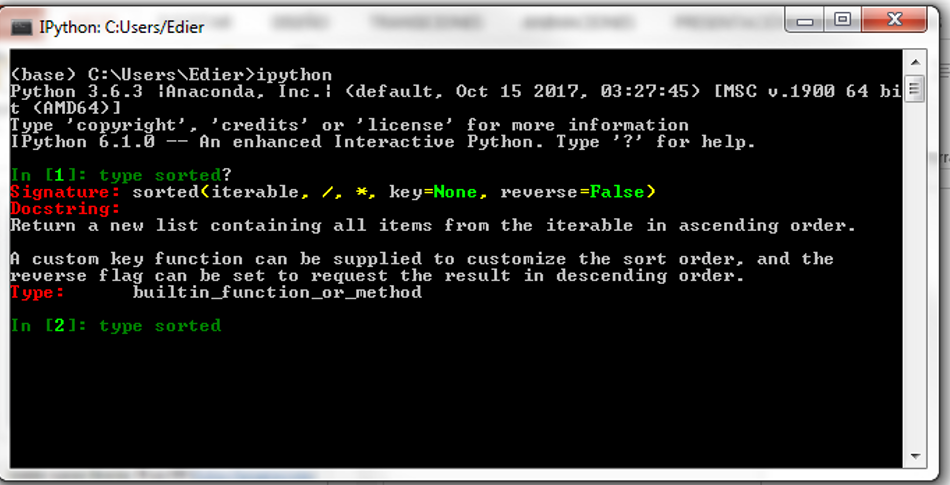
\includegraphics[width=12cm]{ipython}
\end{frame}
%#############################SLIDE 
\begin{frame}
\frametitle{Spyder}
\centering
	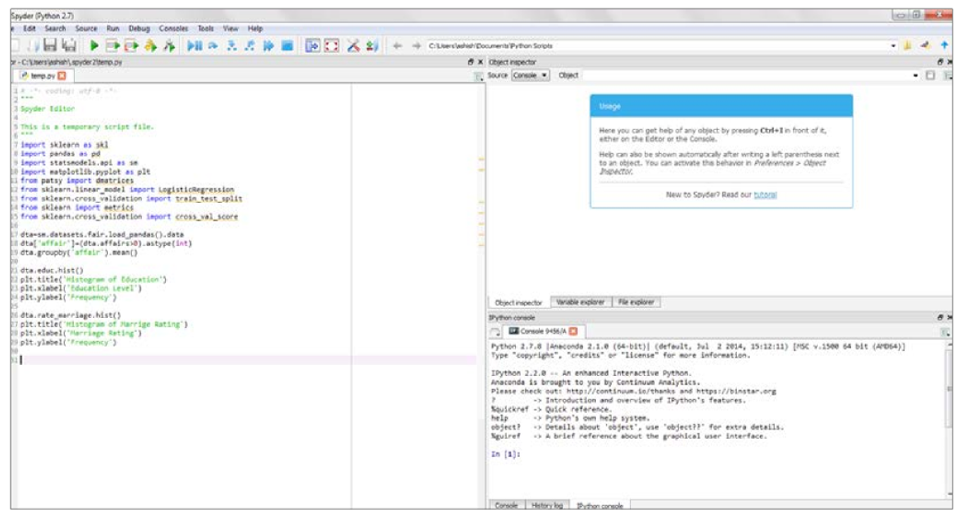
\includegraphics[width=12cm]{spyder}
\end{frame}
%#############################SLIDE 
\begin{frame}
\frametitle{Jupyter Lab}
\framesubtitle{Notebook .ipynb}
\centering
	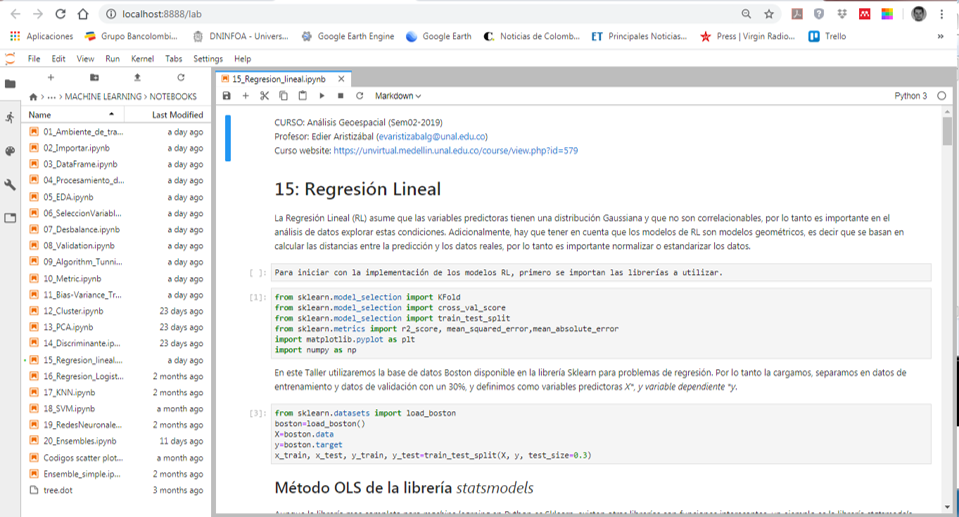
\includegraphics[width=12cm]{jupyterlab}
\end{frame}
%#############################SLIDE 
\end{document} 
 %############################END###################################